\documentclass[17pt]{extarticle}
\usepackage{../mystyle}

\begin{document}
\section*{Работа №4}
\begin{figure}[h!]
    \centering
    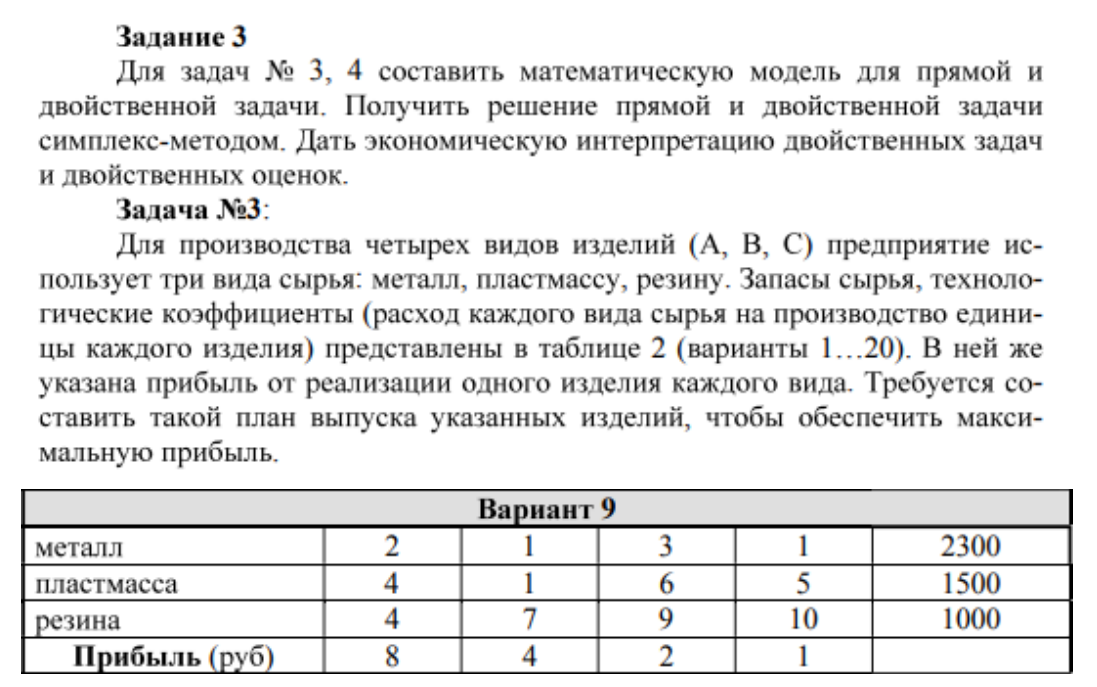
\includegraphics[width=0.7\textwidth]{c.png}
    \caption{Изображение постановки задачи}
\end{figure}

\subsection*{Постановка задачи}

\subsubsection*{Прямая задача}
Найти оптимальный план производства продукции с максимальной прибылью, для которого достаточно имеющихся ресурсов.
\[
    x_1, x_2, x_3, x_4 \text{ — количество произведенной продукции.}
\]
\textbf{Целевая функция}:
\[
    F = 8x_1 + 4x_2 + 2x_3 + 1x_4 \to \max
\]
\textbf{Ограничения}:
\[
    \begin{cases}
        2x_1 + 1x_2 + 3x_3 + 1x_4 \leq 2300  \\
        4x_1 + 1x_2 + 6x_3 + 5x_4 \leq 1500  \\
        4x_1 + 7x_2 + 9x_3 + 10x_4 \leq 1000 \\
        x_1, x_2, x_3, x_4 \geq 0            \\
    \end{cases}
\]

\subsubsection*{Двойственная задача}
Оценить каждый из видов сырья, используемого для производства продукции. Оценки, приписываемые каждому виду сырья, должны быть такими, чтобы оценка всего используемого сырья была минимальна, а суммарная оценка сырья, используемого для производства единицы продукции, — не меньше цены единицы продукции.
\textbf{Целевая функция двойственной задачи}:
\[
    G = 2300y_1 + 1500y_2 + 1000y_3 \to \min
\]
\textbf{Ограничения}:
\[
    \begin{cases}
        2y_1 + 4y_2 + 4y_3 \geq 8  \\
        1y_1 + 1y_2 + 7y_3 \geq 4  \\
        3y_1 + 6y_2 + 9y_3 \geq 2  \\
        1y_1 + 5y_2 + 10y_3 \geq 1 \\
        y_1, y_2, y_3 \geq 0       \\
    \end{cases}
\]

\subsection*{Решим прямую задачу}

\[
    F = 8x_1 + 4x_2 + 2x_3 + 1x_4 + 0x_5 + 0x_6 + 0x_7 \to \max
\]
\[
    \begin{cases}
        2x_1 + 1x_2 + 3x_3 + 1x_4 + 1x_5 + 0x_6 + 0x_7 = 2300  \\
        4x_1 + 1x_2 + 6x_3 + 5x_4 + 0x_5 + 1x_6 + 0x_7 = 1500  \\
        4x_1 + 7x_2 + 9x_3 + 10x_4 + 0x_5 + 0x_6 + 1x_7 = 1000 \\
        x_1, x_2, x_3, x_4 \geq 0                              \\
    \end{cases}
\]

\begin{table}[h!]
    \centering
    \begin{tabular}{c|c|ccccccc|c|c}
        \toprule
        Basis & C base & x1 & x2 & x3 & x4 & x5 & x6 & x7 & B    & reduced\_cost \\
        \midrule
        A5    & 0      & 2  & 1  & 3  & 1  & 1  & 0  & 0  & 2300 & 1150          \\
        A6    & 0      & 4  & 1  & 6  & 5  & 0  & 1  & 0  & 1500 & 375           \\
        A7    & 0      & 4  & 7  & 9  & 10 & 0  & 0  & 1  & 1000 & 250           \\
        \midrule
              & delta  & 8  & 4  & 2  & 1  & 0  & 0  & 0  & 0    &               \\
              & c      & 8  & 4  & 2  & 1  & 0  & 0  & 0  & 0    &               \\
        \bottomrule
    \end{tabular}
\end{table}

\begin{table}[h!]
    \centering
    \begin{tabular}{c|c|ccccccc|c}
        \toprule
        Basis & C base & x1 & x2   & x3   & x4  & x5 & x6 & x7   & B    \\
        \midrule
        A5    & 0      & 0  & -2.5 & -1.5 & -4  & 1  & 0  & -0.5 & 1800 \\
        A6    & 0      & 0  & -6   & -3   & -5  & 0  & 1  & -1   & 500  \\
        A1    & 8.0    & 1  & 1.75 & 2.25 & 2.5 & 0  & 0  & 0.25 & 250  \\
        \midrule
              & delta  & 0  & -10  & -16  & -19 & 0  & 0  & -2   & 2000 \\
              & c      & 8  & 4    & 2    & 1   & 0  & 0  & 0    & 0    \\
        \bottomrule
    \end{tabular}
\end{table}

\[
    x_1 = 250, \ x_5 = 1800, \ x_6 = 500
\]
\[
    \begin{cases}
        1x_2 + 3x_3 + 1x_4 = 0         \\
        1x_2 + 6x_3 + 5x_4 = 0         \\
        7x_2 + 9x_3 + 10x_4 + 1x_7 = 0 \\
    \end{cases}
\]
\[
    \begin{cases}
        1x_2 + 3x_3 + 1x_4 = 0         \\
        3x_3 + 4x_4 = 0                \\
        7x_2 + 9x_3 + 10x_4 + 1x_7 = 0 \\
    \end{cases}
\]
\[
    \begin{cases}
        1x_2 + 3x_3 + -\frac{3}{4}x_3 = 0        \\
        x_4 = -\frac{3}{4}x_3                    \\
        7x_2 + 9x_3 - \frac{30}{4}x_3 + 1x_7 = 0 \\
    \end{cases}
\]
\[
    \begin{cases}
        1x_2 + \frac{9}{4}x_3 = 0        \\
        x_4 = -\frac{3}{4}x_3            \\
        7x_2 + \frac{6}{4}x_3 + 1x_7 = 0 \\
    \end{cases}
\]
\[
    F_{\text{max}} = 2000 = 8 \cdot 250 + 4x_2 + 2x_3 + x_4 = 2000 + 4x_2 + \frac{5}{4}x_3 \\
    \Rightarrow 4x_2 + \frac{5}{4}x_3 = 0
\]
\[
    \begin{cases}
        1x_2 + \frac{9}{4}x_3 = 0        \\
        4x_2 + \frac{5}{4}x_3 = 0        \\
        7x_2 + \frac{6}{4}x_3 + 1x_7 = 0 \\
        x_4 = -\frac{3}{4}x_3            \\
    \end{cases}
\]
\[
    \begin{cases}
        x_1 = 250                 \\
        x_5 = 1800                \\
        x_6 = 500                 \\
        x_2 = x_3 = x_4 = x_7 = 0 \\
    \end{cases}
\]
\[
    F_{\text{max}} = 2000
\]

\subsection*{Решим обратную задачу}

\[
    \begin{split}
        y^* =
        \begin{pmatrix}
            0 & 0 & 8
        \end{pmatrix}
        \cdot
        \begin{pmatrix}
            1 & 0 & -0.5 \\
            0 & 1 & -1   \\
            0 & 0 & 0.25
        \end{pmatrix}
        = (0, 0, 2) \\
        G_{\text{min}} = 2300 \cdot 0 + 1500 \cdot 0 + 1000 \cdot 2 = 2000 = F_{\text{max}}
    \end{split}
\]

Видим, что первый и второй материал в избытке, третий материал дефицитный.
\[
    \begin{cases}
        2 \cdot 0 + 4 \cdot 0 + 4 \cdot 2 = 8  \\
        1 \cdot 0 + 1 \cdot 0 + 7 \cdot 2 > 4  \\
        3 \cdot 0 + 6 \cdot 0 + 9 \cdot 2 > 2  \\
        1 \cdot 0 + 5 \cdot 0 + 10 \cdot 2 > 1 \\
    \end{cases}
\]

Первое ограничение выполняется как равенство
\(\Rightarrow\)
двойственные оценки ресурсов, используемых для производства единицы продукции A, равны в точности доходам
\(\Rightarrow\)
производить это изделие целесообразно (\(x^*_1 = 250\)).

Второе, третье и четвертое ограничения выполняются как больше
\(\Rightarrow\) производить изделия B, C и S экономически невыгодно
\[
    x^*_2 = 0, x^*_3 = 0, x^*_4 = 0
\]

\subsection*{Анализ устойчивости двойственных оценок}

\[
    \begin{split}
        x^*_b = x_b + A^{-1}_b \cdot (b + \Delta b) \\
        A^{-1}_b \cdot (b + \Delta b) = \\
        \begin{pmatrix}
            1 & 0 & -0.5 \\
            0 & 1 & -1   \\
            0 & 0 & 0.25
        \end{pmatrix}
        \cdot
        \begin{pmatrix}
            2300 + \Delta b_1 \\
            1500 + \Delta b_2 \\
            1000 + \Delta b_3 \\
        \end{pmatrix}
        = \\
        \begin{pmatrix}
            1800 + \Delta b_1 - 0.5 \Delta b_3 \\
            500 + \Delta b_2 - \Delta b_3      \\
            250 + 0.25 \Delta b_3              \\
        \end{pmatrix} \geq 0 \\
        1) \Delta b_2 = \Delta b_3 = 0 \Rightarrow \Delta b_1 \in [-1800, +\infty) \\
        2) \Delta b_1 = \Delta b_3 = 0 \Rightarrow \Delta b_2 \in [-500, +\infty) \\
        3) \Delta b_1 = \Delta b_2 = 0 \Rightarrow \Delta b_3 \in [-1000, 500] \\
    \end{split}
\]

Предположим: \(\Delta b_2 = -100; \Delta b_3 = -200\)

\[
    \begin{split}
        \begin{pmatrix}
            1800 - 0.5 \cdot (-200) \\
            500 - (-200)            \\
            250 + 0.25 \cdot (-200) \\
        \end{pmatrix} =
        \begin{pmatrix}
            1900 \\
            700  \\
            200  \\
        \end{pmatrix} \geq 0 \\
        x^*_b = \begin{pmatrix}
            1800 + 1900 \\
            500 + 700   \\
            250 + 200   \\
        \end{pmatrix} = \begin{pmatrix}
            3700 \\
            1200 \\
            450  \\
        \end{pmatrix} \\
        F^* = 8 \cdot 3700 + 4 \cdot 1200 + 2 \cdot 450 + 1 \cdot 450 = 5750
    \end{split}
\]

Видим, что прибыль увеличилась.

\end{document}